%%=============================================================================
%% Conclusie
%%=============================================================================

\chapter{Conclusie}%
\label{ch:conclusie}

% onderzoeksvra(a)g(en). Wat was jouw bijdrage aan het onderzoeksdomein en
% hoe biedt dit meerwaarde aan het vakgebied/doelgroep? 
% Reflecteer kritisch over het resultaat. In Engelse teksten wordt deze sectie
% ``Discussion'' genoemd. Had je deze uitkomst verwacht? Zijn er zaken die nog
% niet duidelijk zijn?
% Heeft het onderzoek geleid tot nieuwe vragen die uitnodigen tot verder 
%onderzoek?
\subsubsection{Inleiding}
In dit hoofdstuk zal er getracht worden een conclusie te formuleren op de hoofdonderzoeksvraag en diens subvragen.

\section{Subonderzoeksvraag 1}
Na het opstellen van de proof-of-concept werden er metingen uitgevoerd op zowel het bestaande systeem als de proof-of-concept. Dit met als doel een conclusie op de eerste subonderzoeksvraag, namelijk: ``Wat is de gemiddelde reactiesnelheid van de .NET MAUI applicatie en hoe verhoudt deze zich ten opzichte van de gemiddelde reactiesnelheid van het huidige systeem?''

De hypothese voor deze vraag luidt als volgt: ``de gemiddelde reactietijd van de POC is kleiner dan de gemiddelde reactietijd van de huidige applicatie''

Om de hypothese te kunnen aannemen of verwerpen werden enkele statistische toetsen uitgevoerd:

\begin{enumerate}
    \item Het gemiddelde van de twee datasets werd berekend
    
    \begin{itemize}
        \item Voor het huidige systeem is het gemiddelde gelijk aan 1867,076
        
        \item Voor de proof-of-concept is het gemiddelde gelijk aan 523,931
    \end{itemize}

    Hieruit kan al geconcludeerd worden dat de gemiddelde reactiesnelheid van de proof-of-concept veel lager is dan de reactiesnelheid van het huidig systeem.

    \item Een twee-sample T-test werd uitgevoerd. Deze test zou een definitief antwoord moeten geven over de geldigheid van de hypothese. Voor deze test werd een significantieniveau van 0,05 gebruikt. Daarnaast werden ook twee hypotheses opgesteld, namelijk:
    
    \begin{itemize}
        \item H0: de gemiddelde reactietijd van de POC is groter of gelijk aan de gemiddelde reactietijd van de huidige applicatie
        
        \item H1: de gemiddelde reactietijd van de POC is kleiner dan de gemiddelde reactietijd van de huidige applicatie
    \end{itemize}

    Na het uitvoeren van deze test werd een p-waarde, ook wel de overschrijdingskans genoemd, vastgesteld die ongeveer gelijk was aan nul. Aangezien de p-waarde kleiner is dan het bovengenoemde significantieniveau, mag de nulhypothese verworpen worden.
\end{enumerate}

Kortom beide statistische proeven tonen aan dat de initiële hypothese klopt. Daarnaast kan er dankzij deze twee proeven ook een antwoord op de onderzoeksvraag geformuleerd worden, namelijk: de gemiddelde reactiesnelheid van de .NET MAUI-applicatie is gelijk aan 523,931 en is in verhouding tot het huidig systeem 3,56 keer zo snel op vlak van reactietijd.

\begin{figure}[H]
    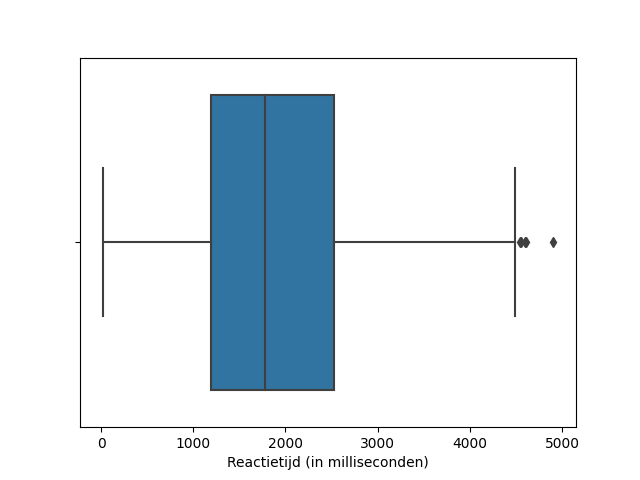
\includegraphics{Current_Plot_Boxplot}
    \centering
    \caption{Boxplot van de reactietijden in het huidige syteem}
    \label{fig:httpLongPolling}
\end{figure}

\begin{figure}[H]
    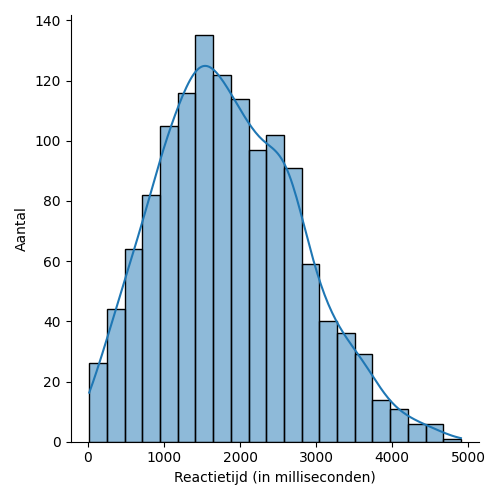
\includegraphics{Current_Plot_Histogram}
    \centering
    \caption{Histogram van de reactietijden in het huidige syteem}
    \label{fig:httpLongPolling}
\end{figure}

\begin{figure}[H]
    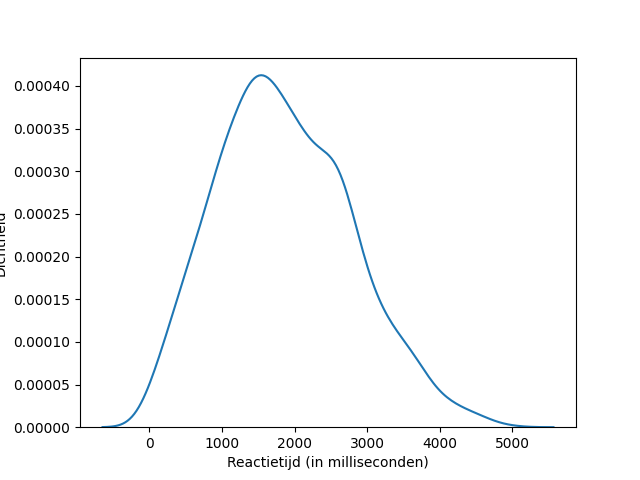
\includegraphics{Current_Plot_Density}
    \centering
    \caption{Densiteitsgrafiek van de reactietijden in het huidige sysyteem}
    \label{fig:httpLongPolling}
\end{figure}

\begin{figure}[H]
    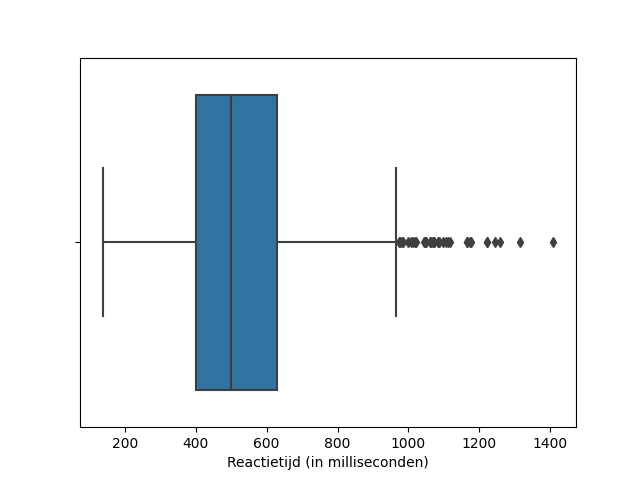
\includegraphics{POC_Plot_Boxplot}
    \centering
    \caption{Boxplot van de reactietijden in de proof-of-concept}
    \label{fig:httpLongPolling}
\end{figure}

\begin{figure}[H]
    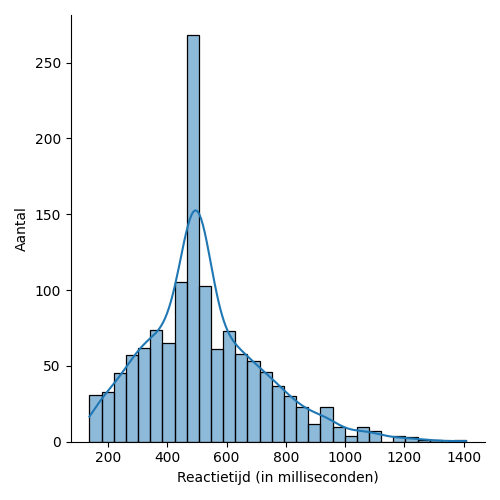
\includegraphics{POC_Plot_Histogram}
    \centering
    \caption{Histogram van de reactietijden in de proof-of-concept}
    \label{fig:httpLongPolling}
\end{figure}

\begin{figure}[H]
    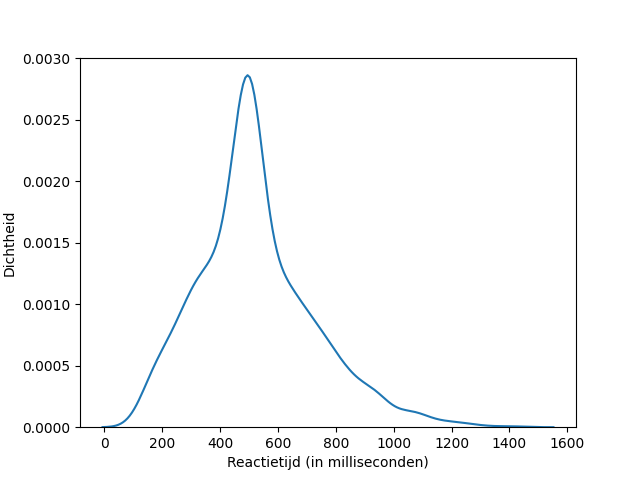
\includegraphics{POC_Plot_Density}
    \centering
    \caption{Densiteitsgrafiek van de reactietijden in de proof-of-concept}
    \label{fig:httpLongPolling}
\end{figure}

\section{Subonderzoeksvraag 2}
Het tweede luik van de onderzoeksvraag luidt als volgt: ``Laat .NET MAUI het toe om push-notificatie te versturen?''

.NET MAUI levert geen algemene bibliotheek aan om push-notificaties te implementeren in de mobiele applicaties. Om dit te kunnen verwezenlijken, moeten we voor ieder platform een verschillend project opzetten die enkel de applicatie voor dat platform kan gaan bouwen. Daarnaast is er ook nood aan het gebruik van een bibliotheek uitgegeven door een derde partij. In dit geval gaat het om de Plugin.Firebase biblitoheek gemaakt en onderhouden door Tobias Buchholz. Dit zorgt ervoor dat de applicatie moet steunen op Firebase, wat een verzameling is van backend cloud computing services aangeboden door Google.

Dit alles zorgt ervoor dat er geconludeerd kan worden dat .NET MAUI het wel toelaat om push-notificaties te versturen, maar dat dit niet eenmalig geïmplementeerd kan worden voor de drie platformen samen. Dit zorgt er dan ook voor dat enkele van de voordelen van een cross-platform framework wegvallen.

\section{Algemene conclusie}
Door de conclussies geformuleerd voor de twee subonderzoeksvragen kan nu ook een algemeen besluit gevormd worden. Zoals in de inleiding wordt vermeld is het onderzoek een partiëel succes wanneer een positief besluit gevormd kan worden voor de eerste subonderzoeksvraag. Deze proef is een compleet succes wanneer de tweede subonderzoeksvraag een positief resultaat verkrijgt.

Dit onderzoek is alvast een partiëel succes aangezien het antwoord op de vraag: ``Wat is de gemiddelde reactiesnelheid van de .NET MAUI applicatie en hoe verhoudt deze zich ten opzichte van de gemiddelde reactiesnelheid van het huidige systeem?'' als volgt luidt: ``De gemiddelde reactiesnelheid van .NET MAUI is gelijk aan 523,931 en is in verhouding tot de gemiddelde reactiesnelheid van het huidige systeem 3,56 keer zo snel''.

Over het complete succes van de proef kan gedebateerd worden aangezien het mogelijk is om push-notificaties te versturen. Echter is dit momenteel enkel mogelijk indien er voor de verschillende platformen een aparte codebase wordt gebouwd (wat indruist tegen de visie van .NET MAUI) en er geen standaard bibliotheken aangeleverd worden door Microsoft. In deze proef wordt dit dan ook niet aanzien als een succes.

Dit alles zorgt er voor dat de algemene conclusie van deze proef als volgt luidt: .NET MAUI is voldoende matuur om een POS-systeem geschreven in COBOL te vervangen. Echter wanneer nood is aan het gebruik van niche features, zoals bijvoorbeeld het gebruik van push-notificaties, heeft .NET MAUI nog wat zaken die (beter) geïmplementeerd moeten worden.